% Created 2016-08-17 Wed 14:38
\documentclass[tikz]{standalone}

\usepackage[utf8]{inputenc}
\usepackage[T1]{fontenc}

\usepackage{circledsteps}

\RequirePackage{xcolor}

%% HPI color definitions according to the design manual
% These do not exactly match the RGB values used in the Powerpoint slide master due to unknown reasons
\definecolor{hpiyellow}{RGB}{246,168,0}
\definecolor{hpiorange}{RGB}{221,97,8}
\definecolor{hpired}{RGB}{177,6,58}
\definecolor{hpigray}{RGB}{90,96,101}
\definecolor{hpiblue}{RGB}{0,122,158}


\renewcommand{\sfdefault}{neosans}
% Different font weights for neosans
\newcommand{\textl}[1]{{\fontseries{l}\selectfont #1}} % light
\newcommand{\textm}[1]{{\fontseries{m}\selectfont #1}} % medium, same as default weight
\newcommand{\textsb}[1]{{\fontseries{sb}\selectfont #1}} % semibold
\newcommand{\textmb}[1]{{\fontseries{mb}\selectfont #1}} % bold, same as \textbf
\newcommand{\texteb}[1]{{\fontseries{eb}\selectfont #1}} % extra bold
\newcommand{\textub}[1]{{\fontseries{ub}\selectfont #1}} % ultra bold

\tikzset{every picture/.style={/utils/exec={\sffamily}}}
\tikzset{flipflop RSflanke/.style={
  flipflop,
  flipflop def={t1=S, t2=C, c2=1, t3=R, t6=Q, t4={\ctikztextnot{Q}}}
}}


\tikzset{
  mechanicalSwitch/.pic={
    \coordinate (-inUp) at (135:2); 
    \coordinate (-inDown) at (235:2);
    \coordinate (-out) at (2,0);
    \coordinate (-center) at (0,0);
    
    \draw (0,0) circle [radius = 2cm];
    \draw [fill=gray!20] (0,0) circle [radius = 0.2cm];

    \draw (0, 0) -- (2, 0);
    \draw (135:.8) -- (135:2); 
    \draw (225:.8) -- (225:2); 

    \draw [fill=gray!20] (2, 0) circle [radius=0.05cm]; 
    \draw [fill=gray!20] (135:2) circle [radius=0.05cm]; 
    \draw [fill=gray!20] (225:2) circle [radius=0.05cm]; 

    
    \draw [thick] (0,0) -- (175:1.5); 

    \draw [dashed, <->, domain=135:225] plot ({cos(\x)}, {sin(\x)}); 
  },
  mechanicalSwitchClosed/.pic={
    \coordinate (-inUp) at (135:2); 
    \coordinate (-inDown) at (255:2);
    \coordinate (-out) at (2,0);
    \coordinate (-center) at (0,0);
    \draw (0,0) circle [radius = 2cm];
    \draw [fill=gray!20] (0,0) circle [radius = 0.2cm];

    \draw (0, 0) -- (2, 0);
    \draw (135:.8) -- (135:2); 
    \draw (225:.8) -- (225:2); 

    \draw [fill=gray!20] (2, 0) circle [radius=0.05cm]; 
    \draw [fill=gray!20] (135:2) circle [radius=0.05cm]; 
    \draw [fill=gray!20] (225:2) circle [radius=0.05cm]; 

    
    \draw [thick] (0,0) -- (135:2); 

    \draw [dashed, <->, domain=135:225] plot ({cos(\x)}, {sin(\x)}); 
  }
}


\usetikzlibrary{calc}
\usetikzlibrary{positioning}


\usepackage{tikzpeople}
\usetikzlibrary {shapes.symbols,shapes.geometric}
\usepackage{bytefield}

\begin{document}

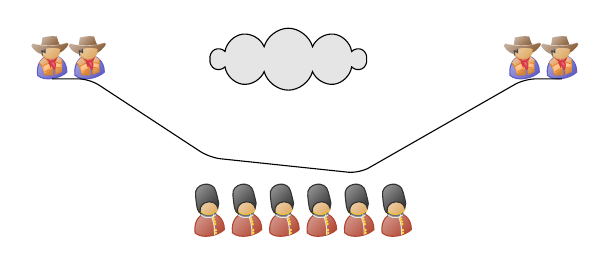
\begin{tikzpicture}
  \label{page:transport:two_army}

  \node [cowboy] (c1) at (-3, 2)  {}; 
  \node [cowboy, right=0.1cm of c1] (c2) {}; 
  \node [cowboy] (c3) at (3, 2)  {}; 
  \node [cowboy, right=0.1cm of c3] (c4) {}; 


  \node [guard] (g1) at (-1, 0)  {}; 
  \node [guard, right=0.1cm of g1] (g2)  {}; 
  \node [guard, right=0.1cm of g2] (g3)  {}; 
  \node [guard, right=0.1cm of g3] (g4)  {}; 
  \node [guard, right=0.1cm of g4] (g5)  {}; 
  \node [guard, right=0.1cm of g5] (g6)  {}; 

  \draw [rounded corners] (c1.south) -- (c2.south) -- ([shift={(0,.5)}]  g1.north) -- ([shift={(0,.3)}] g5.north) -- (c3.south) -- (c4.south);


  \node [cloud, draw, aspect=6, fill=gray!20] at (0, 2) {};
\end{tikzpicture}


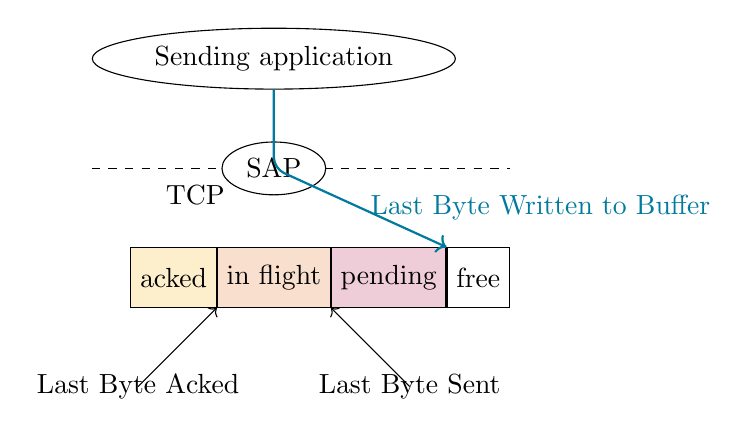
\begin{tikzpicture}
  \label{page:transport:send_buffer}

  \node [ellipse, draw] (sender){Sending application};


  
  \node [draw, minimum height=5ex, fill=hpiorange!20, below=2cm of sender] (inflight)  { in flight}; 
  \node [draw, minimum height=5ex, fill=hpiyellow!20, left=0cm of inflight] (acked)  { acked }; 
  \node [draw, minimum height=5ex, fill=hpired!20, right=0cm of inflight] (pending)  { pending }; 
  \node [draw, minimum height=5ex, fill=white!20, right=0cm of pending] (free)  { free }; 

  \coordinate (sap) at ($(sender.south)!0.5!(inflight.north)$);

  \draw [dashed] (sap -| sender.west) -- (sap -| free.east); 
  \node [ellipse, draw, fill=white] at (sap) (sapnode)  {SAP}; 
  \node [anchor=north east,below left=0.1cm and 0.5cm of sap.south west] (tcp)  {TCP}; 
  
  \draw [hpiblue, thick, ->, rounded corners] (sender.south) -- (sap) to node[right] {Last Byte Written to Buffer} (pending.north east);

  \draw [<-] (acked.south east) -- ++ (-1, -1) node {Last Byte Acked}; 
  \draw [<-] (inflight.south east) -- ++ (+1, -1) node {Last Byte Sent}; 

  
\end{tikzpicture}

\begin{tikzpicture}
  \label{page:transport:receiver_buffer}

  \node [ellipse, draw] (sender){Receiving application};


  
  \node [draw, minimum height=5ex, fill=hpiorange!20, below=2cm of sender] (block1)  { received}; 
  \node [draw, minimum height=5ex, fill=hpiyellow!20, left=0cm of block1] (delivered)  { delivered }; 
  \node [draw, minimum height=5ex, fill=hpired!20, right=0cm of block1] (gap1)  { missing }; 
  \node [draw, minimum height=5ex, fill=hpiorange!20, right=0cm of gap1] (block2)  { also received }; 
  \node [draw, minimum height=5ex, fill=hpired!20, right=0cm of block2] (gap1)  { missing }; 

  \coordinate (sap) at ($(sender.south)!0.5!(inflight.north)$);

  \draw [dashed] (sap -| sender.west) -- (sap -| free.east); 
  \node [ellipse, draw, fill=white] at (sap) (sapnode)  {SAP}; 
  \node [anchor=north east,below left=0.1cm and 0.5cm of sap.south west] (tcp)  {TCP}; 

  \draw [hpiblue, thick, ->, rounded corners] (sender.south) -- (sap) to node[right] {Last Byte Read from Buffer} (delivered.north east);

  \draw [<-] (block1.south east) -- ++ (-1, -1) node {Next Seq.No. Expected}; 
  \draw [<-] (block2.south east) -- ++ (+1, -1) node {Biggest Seq.No. Received}; 

  
\end{tikzpicture}

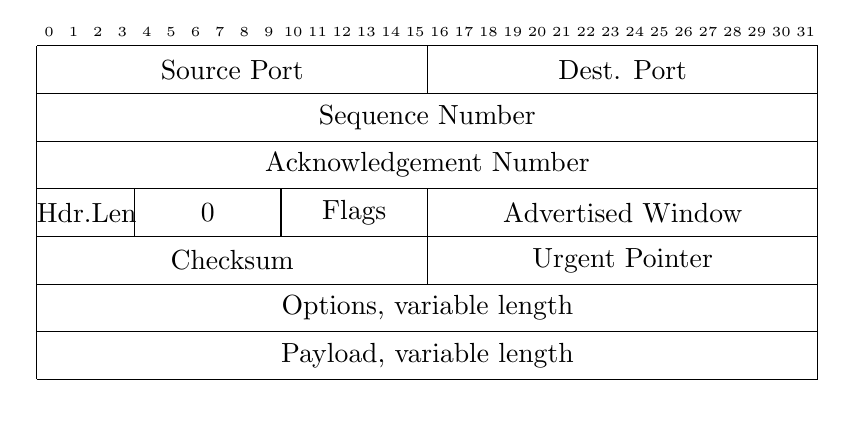
\begin{tikzpicture}
  \label{page:transport:tcp_header}
  \node {
    \begin{bytefield}[endianness=little]{32}
      \bitheader{0-31}\\
      \bitbox{16}{Source Port}
      \bitbox{16}{Dest. Port} \\
      \wordbox{1}{Sequence Number} \\
      \wordbox{1}{Acknowledgement  Number} \\
      \bitbox{4}{Hdr.Len}
      \bitbox{6}{0}
      \bitbox{6}{Flags}
      \bitbox{16}{Advertised Window}
      \\
      \bitbox{16}{Checksum}
      \bitbox{16}{Urgent Pointer }
      \\
      \wordbox{1}{Options, variable length} \\
      \wordbox{1}{Payload, variable length} \\
    \end{bytefield}  
  };
\end{tikzpicture}

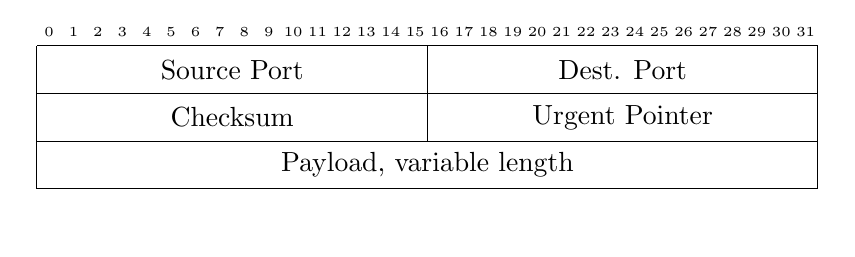
\begin{tikzpicture}
  \label{page:transport:udp_header}
  \node {
    \begin{bytefield}[endianness=little]{32}
      \bitheader{0-31}\\
      \bitbox{16}{Source Port}
      \bitbox{16}{Dest. Port} \\
      \bitbox{16}{Checksum}
      \bitbox{16}{Urgent Pointer }
      \\
      \wordbox{1}{Payload, variable length} \\
    \end{bytefield}  
  };
\end{tikzpicture}






\end{document}